In this section we describe how we have performed the testing of our system.
We have basically followed the guidelines already defined in our Design document so, if you want additional information, please refer to sections 6.4 and 6.5 of that document. \\
As regards ApplicationServer subsystem, since in the DD we have described the testing strategy of the entire planned subsystem, we do not have performed the testing of the entire system but only until event EventManager integration (please refer to our design document to see the order of integration).\\
\begin{figure}[H]
	\begin{center}
		\hspace*{-40pt}
		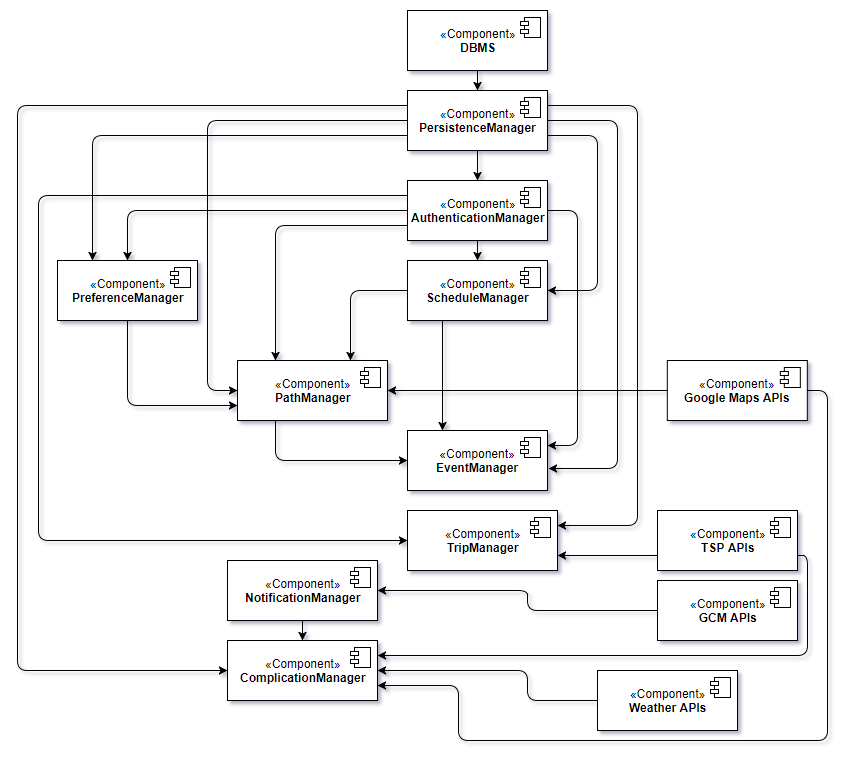
\includegraphics[scale=0.4]{app_server_I&T.png}
	\end{center}
\caption{ ApplicationServer - Actually tested subsystems subsystems}
\end{figure}
\newpage \noindent
For what concerns the Android App subsystem we have tested the DAOs that interact with the local DB. These tests can be found in test/java/it/polimi/travlendarplus, as can be seen in the previous chapter (see section 4.1).

\section{Procedure Adopted}
\subsection{Persistence manager (JPA - DBMS interaction): Arquillian}
In order to perform our \textit{PersistenceManager}'s testing we have adopted the following procedure: we have exploited Arquillian features to obtain a testing configuration that allow us to use a testing container of GlassFish that can run and connect to an embedded GlassFish 3.1 instance.
Our \textit{PersistenceManager}'s tests simply  persist a set of sample entities to the database, connected with the GlassFish container, and then retrieve them using JPA Criteria API.
Each test method checks that the sample data retrieved from the database is correct. Before and after a test is performed, the database is cleaned up, in order to guarantee that each test is run in a clean environment.
This is the outcome of these tests:
\begin{figure}[H]
	\begin{center}
		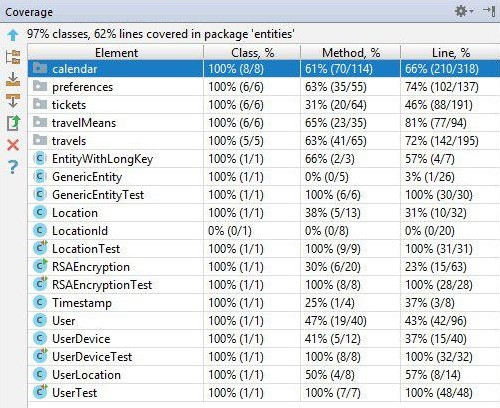
\includegraphics[scale=0.7]{JPA_test_outcome.jpg}
	\end{center}
\caption{ \textit{PersistenceManager} - code coverage}
\end{figure}

\subsection{Enterprise Java Beans: Mockito}
We used Mockito to test the \textit{PathManager}, a Stateless EJB that requires other Stateless EJBs (\textit{ScheduleManager} and \textit{PreferenceManager}) in order to perform its tasks. Making use of Mockito, all the functions performed by one of the injected beans were mocked: the idea is to consider these functions as working and to test the instructions properly defined in the \textit{PathManager}. 
\newpage
In particular, we mocked \textit{ScheduleManager} functions in this way:
\begin{itemize}
	\item for each function that returns an event a predefined event is returned, depending on the parameter passed to the function;
	\item for \textit{PathCalculation} function a random response is returned, based on the travels passed to the function;
	\item for save functions a \textit{doNothing} method is used.
\end{itemize}  
\textit{PreferenceManager} functions are mocked in this way:
\begin{itemize}
	\item \textit{checkConstraints} function return always \textit{true};
	\item \textit{findBestPath} function return always the first element in the array of possibilities.
\end{itemize}
The most challenging functionalities that our system offers are the calculation of feasible paths, related to the events, that respect the user's constraints and  the possibility to force not scheduled events into the user's schedule. \\ \\
\textit{CalculatePath} function, for a given event, returns the path that allows the user to reach his event and the path that allows him to reach also the following one, according to the commitments in the schedule. \\
We considered a general case in which both previous and following events exist, we verified that:

\begin{itemize}
	\item when an event is inserted and the allotted time between the previous event and the inserted one is enough, we expect to obtain a feasible path;
	\item when an event is inserted and the allotted time between the inserted event and the following one is enough, we expect to obtain a feasible path;
	\item when an event preference ask that the feasible path starts from the precedent user's location (location of the previous event) we expect to obtain a path that starts form there;
	\item when an event preference ask that the feasible path starts from a given location (specified by the user) we expect to obtain a path that starts form there;
	\item for every obtained path, related to a given event, we always expect that the path's ending location is the same as the event location.
\end{itemize}
\noindent
All the previous test cases are checked for the inserted event and its following one (since when an event is inserted the following path can change). When a following event does not exists the following path does not exist and so it has not to be checked. \\ \\
\noindent
We tested also \textit{swapEvents} function, a function that forces an overlapping event into the schedule and removes from the schedule all the events in conflict with the added one. \\
We verified the right behavior of the function in the following cases:
\begin{itemize}
	\item when the forced event overlaps with another one, the latter has to be removed from the schedule;
	\item when the forced event's path overlaps with another event, the conflicting event has to be removed from the schedule;
	\item when the forced event is inserted into the schedule and the following one is too close in time (and so a feasible path does not exist anymore), the following one has to be removed from the schedule;
	\item when the forced event is inserted into the schedule and it overlaps with a break event, but its minimum time is still guaranteed, the break event must remain into the schedule;
	\item when the forced event is inserted into the schedule and it overlaps with a break event, whose minimum time is no more guaranteed, the break event must be removed from the schedule. \\
\end{itemize}
We used Junit in order to test the beans that don't contain components difficult to test.
\begin{figure}[H]
	\begin{center}
		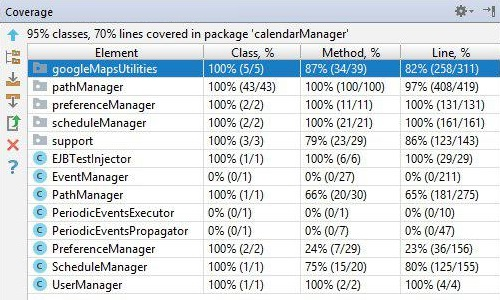
\includegraphics[scale=0.7]{CalendarManager_test_outcome.jpg}
	\end{center}
\caption{ textit{CalendarManager} - code coverage}
\end{figure}

\subsection{RESTful API Postman}
In order to test our RESTful APIs we have performed our requests using an useful software tools Postman. This software tool had allow us to build API requests and see their outcome, checking that:
\begin{itemize}
	\item all invalid (due to wrong message format) requests are refused;
	\item all requests that tries to access secured resources without being authenticated (with a token) receive an unauthorized response message;
	\item all requests with a right message format but with invalid syntax receive a bad request response message;
	\item all the correct requests gets replied with the correct response message. 
\end{itemize}
(For additional info about our RESTful API please refer to our relative documentation \href{httpsdocumenter.getpostman.comview2934379travlendar-restful-api7Log3CL}{\color{blue}link}).


